%  LaTeX support: latex@mdpi.com 
%  For support, please attach all files needed for compiling as well as the log file, and specify your operating system, LaTeX version, and LaTeX editor.

%=================================================================
\documentclass[gene,journal,article,submit,moreauthors,pdftex]{Definitions/mdpi} 
\usepackage{natbib}
% For posting an early version of this manuscript as a preprint, you may use "preprints" as the journal and change "submit" to "accept". The document class line would be, e.g., \documentclass[preprints,article,accept,moreauthors,pdftex]{mdpi}. This is especially recommended for submission to arXiv, where line numbers should be removed before posting. For preprints.org, the editorial staff will make this change immediately prior to posting.

%--------------------
% Class Options:
%--------------------
%----------
% journal
%----------
% Choose between the following MDPI journals:
% acoustics, actuators, addictions, admsci, adolescents, aerospace, agriculture, agriengineering, agronomy, ai, algorithms, allergies, analytica, animals, antibiotics, antibodies, antioxidants, appliedchem, applmech, applmicrobiol, applnano, applsci, arts, asi, atmosphere, atoms, audiolres, automation, axioms, batteries, bdcc, behavsci, beverages, biochem, bioengineering, biologics, biology, biomechanics, biomedicines, biomedinformatics, biomimetics, biomolecules, biophysica, biosensors, biotech, birds, bloods, brainsci, buildings, businesses, cancers, carbon, cardiogenetics, catalysts, cells, ceramics, challenges, chemengineering, chemistry, chemosensors, chemproc, children, civileng, cleantechnol, climate, clinpract, clockssleep, cmd, coatings, colloids, compounds, computation, computers, condensedmatter, conservation, constrmater, cosmetics, crops, cryptography, crystals, curroncol, cyber, dairy, data, dentistry, dermato, dermatopathology, designs, diabetology, diagnostics, digital, disabilities, diseases, diversity, dna, drones, dynamics, earth, ebj, ecologies, econometrics, economies, education, ejihpe, electricity, electrochem, electronicmat, electronics, encyclopedia, endocrines, energies, eng, engproc, entropy, environments, environsciproc, epidemiologia, epigenomes, fermentation, fibers, fire, fishes, fluids, foods, forecasting, forensicsci, forests, fractalfract, fuels, futureinternet, futuretransp, futurepharmacol, futurephys, galaxies, games, gases, gastroent, gastrointestdisord, gels, genealogy, genes, geographies, geohazards, geomatics, geosciences, geotechnics, geriatrics, hazardousmatters, healthcare, hearts, hemato, heritage, highthroughput, histories, horticulturae, humanities, hydrogen, hydrology, hygiene, idr, ijerph, ijfs, ijgi, ijms, ijns, ijtm, ijtpp, immuno, informatics, information, infrastructures, inorganics, insects, instruments, inventions, iot, j, jcdd, jcm, jcp, jcs, jdb, jfb, jfmk, jimaging, jintelligence, jlpea, jmmp, jmp, jmse, jne, jnt, jof, joitmc, jor, journalmedia, jox, jpm, jrfm, jsan, jtaer, jzbg, kidney, land, languages, laws, life, liquids, literature, livers, logistics, lubricants, machines, macromol, magnetism, magnetochemistry, make, marinedrugs, materials, materproc, mathematics, mca, measurements, medicina, medicines, medsci, membranes, metabolites, metals, metrology, micro, microarrays, microbiolres, micromachines, microorganisms, minerals, mining, modelling, molbank, molecules, mps, mti, nanoenergyadv, nanomanufacturing, nanomaterials, ncrna, network, neuroglia, neurolint, neurosci, nitrogen, notspecified, nri, nursrep, nutrients, obesities, oceans, ohbm, onco, oncopathology, optics, oral, organics, osteology, oxygen, parasites, parasitologia, particles, pathogens, pathophysiology, pediatrrep, pharmaceuticals, pharmaceutics, pharmacy, philosophies, photochem, photonics, physchem, physics, physiolsci, plants, plasma, pollutants, polymers, polysaccharides, proceedings, processes, prosthesis, proteomes, psych, psychiatryint, publications, quantumrep, quaternary, qubs, radiation, reactions, recycling, regeneration, religions, remotesensing, reports, reprodmed, resources, risks, robotics, safety, sci, scipharm, sensors, separations, sexes, signals, sinusitis, smartcities, sna, societies, socsci, soilsystems, solids, sports, standards, stats, stresses, surfaces, surgeries, suschem, sustainability, symmetry, systems, taxonomy, technologies, telecom, textiles, thermo, tourismhosp, toxics, toxins, transplantology, traumas, tropicalmed, universe, urbansci, uro, vaccines, vehicles, vetsci, vibration, viruses, vision, water, wevj, women, world 

%---------
% article
%---------
% The default type of manuscript is "article", but can be replaced by: 
% abstract, addendum, article, book, bookreview, briefreport, casereport, comment, commentary, communication, conferenceproceedings, correction, conferencereport, entry, expressionofconcern, extendedabstract, datadescriptor, editorial, essay, erratum, hypothesis, interestingimage, obituary, opinion, projectreport, reply, retraction, review, perspective, protocol, shortnote, studyprotocol, systematicreview, supfile, technicalnote, viewpoint, guidelines, registeredreport, tutorial
% supfile = supplementary materials

%----------
% submit
%----------
% The class option "submit" will be changed to "accept" by the Editorial Office when the paper is accepted. This will only make changes to the frontpage (e.g., the logo of the journal will get visible), the headings, and the copyright information. Also, line numbering will be removed. Journal info and pagination for accepted papers will also be assigned by the Editorial Office.

%------------------
% moreauthors
%------------------
% If there is only one author the class option oneauthor should be used. Otherwise use the class option moreauthors.

%---------
% pdftex
%---------
% The option pdftex is for use with pdfLaTeX. If eps figures are used, remove the option pdftex and use LaTeX and dvi2pdf.

%=================================================================
% MDPI internal commands
\firstpage{1} 
\makeatletter 
\setcounter{page}{\@firstpage} 
\makeatother
\pubvolume{1}
\issuenum{1}
\articlenumber{0}
\pubyear{2021}
\copyrightyear{2020}
%\externaleditor{Academic Editor: Firstname Lastname} % For journal Automation, please change Academic Editor to "Communicated by"
\datereceived{} 
\dateaccepted{} 
\datepublished{} 
\hreflink{https://doi.org/} % If needed use \linebreak
%------------------------------------------------------------------
% The following line should be uncommented if the LaTeX file is uploaded to arXiv.org
%\pdfoutput=1

%=================================================================
% Add packages and commands here. The following packages are loaded in our class file: fontenc, inputenc, calc, indentfirst, fancyhdr, graphicx, epstopdf, lastpage, ifthen, lineno, float, amsmath, setspace, enumitem, mathpazo, booktabs, titlesec, etoolbox, tabto, xcolor, soul, multirow, microtype, tikz, totcount, changepage, paracol, attrib, upgreek, cleveref, amsthm, hyphenat, natbib, hyperref, footmisc, url, geometry, newfloat, caption

%=================================================================
%% Please use the following mathematics environments: Theorem, Lemma, Corollary, Proposition, Characterization, Property, Problem, Example, ExamplesandDefinitions, Hypothesis, Remark, Definition, Notation, Assumption
%% For proofs, please use the proof environment (the amsthm package is loaded by the MDPI class).

%=================================================================
% Full title of the paper (Capitalized)
\Title{A modelling strategy to improve cacao quality and productivity }

% MDPI internal command: Title for citation in the left column
\TitleCitation{Title}

% Author Orchid ID: enter ID or remove command
\newcommand{\orcidauthorA}{0000-0000-0000-000X} % Add \orcidA{} behind the author's name
%\newcommand{\orcidauthorB}{0000-0000-0000-000X} % Add \orcidB{} behind the author's name

% Authors, for the paper (add full first names)
\Author{Angela RV $^{1,\dagger,\ddagger}$\orcidA{}, Adriana $^{1,\ddagger}$ and Anyela VCR$^{1,}$*}

% MDPI internal command: Authors, for metadata in PDF
\AuthorNames{Firstname Lastname, Firstname Lastname and Firstname Lastname}

% MDPI internal command: Authors, for citation in the left column
\AuthorCitation{Lastname, F.; Lastname, F.; Lastname, F.}
% If this is a Chicago style journal: Lastname, Firstname, Firstname Lastname, and Firstname Lastname.

% Affiliations / Addresses (Add [1] after \address if there is only one affiliation.)
\address{%
$^{1}$ \quad The John Bingham Laboratory, NIAB, 93 Lawrence Weaver Road, Cambridge CB3 0LE, UK 1; e-mail@e-mail.com\\
$^{2}$ \quad BIOS 2; e-mail@e-mail.com}

% Contact information of the corresponding author
\corres{Correspondence:anyela.camargorodriguez@niab.com; Tel.: (optional; include country code; if there are multiple corresponding authors, add author initials) +xx-xxxx-xxx-xxxx (F.L.)}

% Current address and/or shared authorship
\firstnote{Current address: Affiliation 3} 
\secondnote{These authors contributed equally to this work.}
% The commands \thirdnote{} till \eighthnote{} are available for further notes

%\simplesumm{} % Simple summary

%\conference{} % An extended version of a conference paper

% Abstract (Do not insert blank lines, i.e. \\) 
\abstract{ The aim of this study is predict the best time for harvest cocoa fruits.}

% Keywords
\keyword{ICS95; CCN51; thermal time (List three to ten pertinent keywords specific to the article; yet reasonably common within the subject discipline.)} 

% The fields PACS, MSC, and JEL may be left empty or commented out if not applicable
%\PACS{J0101}
%\MSC{}
%\JEL{}

%%%%%%%%%%%%%%%%%%%%%%%%%%%%%%%%%%%%%%%%%%
% Only for the journal Diversity
%\LSID{\url{http://}}

%%%%%%%%%%%%%%%%%%%%%%%%%%%%%%%%%%%%%%%%%%
% Only for the journal Applied Sciences:
%\featuredapplication{Authors are encouraged to provide a concise description of the specific application or a potential application of the work. This section is not mandatory.}
%%%%%%%%%%%%%%%%%%%%%%%%%%%%%%%%%%%%%%%%%%

%%%%%%%%%%%%%%%%%%%%%%%%%%%%%%%%%%%%%%%%%%
% Only for the journal Data:
%\dataset{DOI number or link to the deposited data set in cases where the data set is published or set to be published separately. If the data set is submitted and will be published as a supplement to this paper in the journal Data, this field will be filled by the editors of the journal. In this case, please make sure to submit the data set as a supplement when entering your manuscript into our manuscript editorial system.}

%\datasetlicense{license under which the data set is made available (CC0, CC-BY, CC-BY-SA, CC-BY-NC, etc.)}

%%%%%%%%%%%%%%%%%%%%%%%%%%%%%%%%%%%%%%%%%%
% Only for the journal Toxins
%\keycontribution{The breakthroughs or highlights of the manuscript. Authors can write one or two sentences to describe the most important part of the paper.}

%%%%%%%%%%%%%%%%%%%%%%%%%%%%%%%%%%%%%%%%%%
% Only for the journal Encyclopedia
%\encyclopediadef{Instead of the abstract}
%\entrylink{The Link to this entry published on the encyclopedia platform.}
%%%%%%%%%%%%%%%%%%%%%%%%%%%%%%%%%%%%%%%%%%
\begin{document}
%%%%%%%%%%%%%%%%%%%%%%%%%%%%%%%%%%%%%%%%%%
%\setcounter{section}{-1} %% Remove this when starting to work on the template.

\section{Introduction}

Cocoa ( \textit{Theobroma cacao }L. ) is an important worldwide perennial tropical crop endemic to the South American rainforests \citep{zuidema2005, motamayor2002, argout2011, Rodriguez2019}. Cacao plant member of the Malvaceae (formerly Sterculiaceae)  botanical family such as  cotton \textit{ Gossypium hirstium} \citep{Nix2017cotton} wich is modeled in SIMPLE model \citep{Zao2019simple}. Cocoa is grown for its fruits, known as cacao pods.  \citep{ Niemenak2010, suarez2021}. Only the 5\% of the world cocoa yield is desalinated for Fine-cocoa production due to the low productivity of  the traditional crop management \citep{argout2011}.  In Colombia, cocoa  is  traditionally  consumed  as  a  beverage. It is one of the crops promoted by the Colombian government in the social and agricultural development  programs aimed at favouring peace in post-conflict regions \citep{Rodriguez2019, Abbott2019} as cocoa is grown by approximately 52.000 \citep{Gutierrez2020} and 98\% of production being carried out by small and medium-sized producers \citep{Garcia2014, Escobar2020}. Colombia registered an increase of 3.750 tons in production in 2020 compared to the previous year \citep{lamos2020}. 

Although Colombian cocoa has the potential to be in the high value markets for fine flavour \citep{Escobar2020}. However, it is still not widely produced as the lack of adoptions of technologies by the traditional farmers. They empirically harvest after 5 or 6 months after flowering date, hence they ferment cocoa beans without considering the  quality of the seeds at the harvest time. This produce heterogeneous characteristics between each fermentation batch diminishing the quality of cocoa final product \citep{Escobar2021}. To identify the best moment to harvest is important to consider physiological responses affected by climate variables such as rain, solar radiation and wind.  Thus,  for cocoa in Colombia, physiological simulation models may be valuable to identify the best moment to harvest cocoa considering variable weather conditions, soil types and cultivar specifications. 

Crop models represent a quantitative assumption of plant growth depending on sunlight interception efficiency values and climate data supported by a large amount of empirical and ground data. \citep{Reynolds2018}. Physiological crop models have shown to be very useful tool for provided agronomical advices and improvements of the cropping systems of annual crops mainly. Recently crop modelling studies are focusing on  perennial crops  production \citep{zuidema2005, Zao2019simple, Bai2020, Romero2021}. However, the information reported  is be less than for annual crops due to the lack of field data available , relatively high research costs and the difficulties of accumulated errors in long-term simulations \citep{zuidema2005}. For cacao there  approaches  to predict yield mainly  using algorithms of machine learning \citep{lamos2020} and just one mechanistic model simulates physiological cocoa performance  "SUCROS-cocoa" \citep{zuidema2005}. This crop model calculates light interception, photosynthesis, maintenance respiration,
evapotranspiration, biomass production and cocoa yield. It can be parametrised having data on cocoa physiology and morphology \citep{zuidema2005}. However,  there is not specific cocoa physiology data available from small and medium-sized producers. Thus, we adapted the simple generic crop model (SIMPLE) that could be easily modified for any crop to simulate development, crop growth and yield using few parameters such as weather and cultivar specification \citep{Zao2019simple}.

In this paper, we present a physiological parametrization of SIMPLE crop model for cocoa to predict the best harvest time  and yield production. We used the SIMPLE crop model \citep{Zao2019simple} for three reasons: 1: That it is very comprehensively described in the original paper. 2: That the code was available in R for initial trials and 3: That it had already been successfully fitted to perennial crops in south America. Overall, the model simulates crop development, growth and yield, and predict the maturation day when the fruit is ready to harvest. It includes 13 parameters ( daily weather data, irrigation, and soil and key dates) to specify a crop type, with four of these for cultivar characteristics easily available from farmer. Thus, this could be used as  tool for small farmers with the aim to improve the quality of cocoa to become more competitive in Fine-cocoa market.
 
%%%%%%%%%%%%%%%%%%%%%%%%%%%%%%%%%%%%%%%%%%
\section{Materials and Methods}
\subsection{Phenology of Cocoa in Colombia}
\begin{figure}[h]
	\centering
	\caption{\footnotesize {Phenology of cocoa in Colombia for crop modelling}} 
	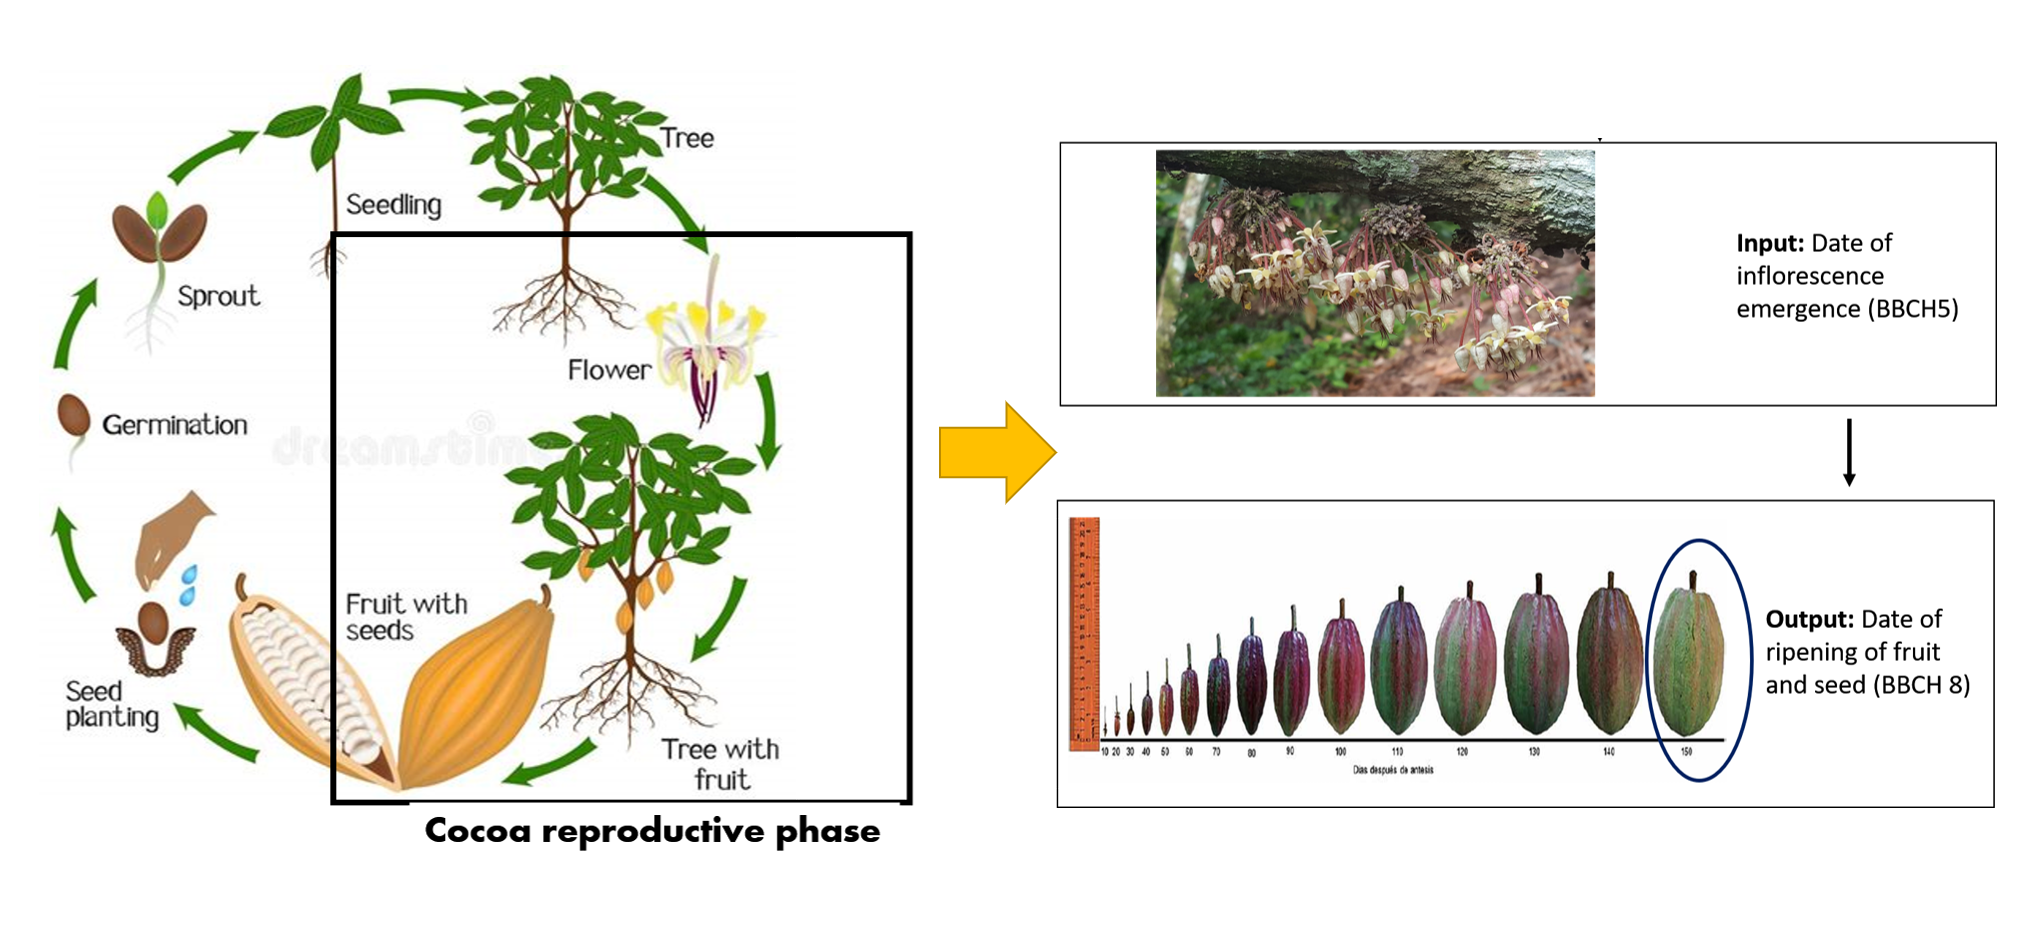
\includegraphics[scale=0.4]{images/phenology.png}\\
	\footnotesize{Credits: Taken from Download from Dreamstime.com, 2021}
	\label{fig:pheno}
\end{figure}.

\subsection{Crop model acquisition}

A zip file of the R codes and input files for the SIMPLE model was kindly provided by Dr Chuang Zhao of the Agricultural and Biological Engineering Department, University of Florida. The main directory contains R codes, the “Parameter definition” Excel ® file, where the units required in each input file for the model are described, instructions and directories containing other input files. Examples of all input files are provided in the Zip files together with a range of data sets that can be used to check model operation after installation. Before running the SimpleB.R program initially line 72 was edited, with RStudio, to provide the full path for the installation. Also, the single year/single experiment mode was selected by setting the GridsimulationSwitch in line 58 to “off” by entering [1] at the end of line 58. After checking the first column in the Input/Simulation Management.csv file is all zeros apart from 1 on line alongside cocoa experiment, then “Source” at the top of the RStudio editing window was clicked. 


In the SIMPLE model dummy files are provided for adding new crop data and weather data, and files 2 to 6 in the list below can be edited to define new cultivars or experiments etc. Then modifying the simulation management file will cause the new files to be read when the program is run.
\begin{enumerate}
	\item Input/Simulation Management.csv
	\item Input/Species parameter.csv
	\item Input/Cultivar.csv
    \item Input/Treatment.csv	
    \item Input/Irrigation.csv
    \item Input/Soil.csv
    \item Observation/Obsdummy crop Exp name.csv	
    \item Weather/dummy weather.WTH
\end{enumerate}

\subsection{Applying the SIMPLE model for the Colombia cocoa crop }

In outline the procedure used was a sequential process of modifying or adding the appropriate files, changing the parameters in the simulation management file, running the program and inspecting the results. This cycle was then repeated until the dry matter yields for Colombia were reasonably reproduced in the results. 
The first step was add the new experiment for cocoa in the dummy crop and experiment names were replaced with our crop and treatment names in the input files and flowering and harvest dates were changed to harvest at 6 months after flowering to check that our modifications could be read. Initially, the new experiment name “KOKOlatl” for the cultivar ICS 95 was used in the species parameter file with other parameters and data founded in papers \textcolor{red}{debo completar eso con la bibliografia de donde saque datos de fisio}, including irrigation, soil features and radiation use efficiency. An appropriate treatment label was added (Figure 7), but all other options pointed to the test data from Brazil.  

\subsection{Input data acquisition } 
Input Weather data were sourced from the POWER Data Access Viewer \citep{nasapower}, which allows automatic download. These were used in as inputs for SIMPLE model. Weather data had to be transformed to .WHT file.


%%%%%%%%%%%%%%%%%%%%%%%%%%%%%%%%%%%%%%%%%%
\section{Results}
\begin{figure}[h]
	\centering
	\caption{\footnotesize {SIMPLE model output for cocoa in Colombia }} 
	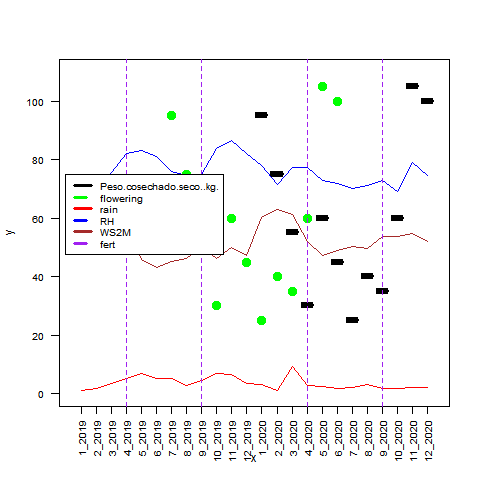
\includegraphics[scale=0.4]{images/averageS.png}\\
	\label{fig:weather}
\end{figure}.

\begin{figure}[h]
	\centering
	\caption{\footnotesize {SIMPLE model output for cocoa in Colombia }} 
	\includegraphics[scale=0.4]{images/outmodel.jpg}\\
	\label{fig:m1}
\end{figure}.

%%%%%%%%%%%%%%%%%%%%%%%%%%%%%%%%%%%%%%%%%%
\section{Discussion}

Authors should discuss the results and how they can be interpreted from the perspective of previous studies and of the working hypotheses. The findings and their implications should be discussed in the broadest context possible. Future research directions may also be highlighted.

Evaluating the level of knowledge of producers regarding cocoa crop management, the harvest was in the group of activities that presented the lowest level of knowledge on the part of the producers according to the general averages \citep{Gutierrez2020}. 

%%%%%%%%%%%%%%%%%%%%%%%%%%%%%%%%%%%%%%%%%%
\section{Conclusions}

This section is not mandatory, but can be added to the manuscript if the discussion is unusually long or complex.

%%%%%%%%%%%%%%%%%%%%%%%%%%%%%%%%%%%%%%%%%%
\section{Patents}

This section is not mandatory, but may be added if there are patents resulting from the work reported in this manuscript.

%%%%%%%%%%%%%%%%%%%%%%%%%%%%%%%%%%%%%%%%%%
\vspace{6pt} 

%%%%%%%%%%%%%%%%%%%%%%%%%%%%%%%%%%%%%%%%%%
%% optional
%\supplementary{The following are available online at \linksupplementary{s1}, Figure S1: title, Table S1: title, Video S1: title.}

% Only for the journal Methods and Protocols:
% If you wish to submit a video article, please do so with any other supplementary material.
% \supplementary{The following are available at \linksupplementary{s1}, Figure S1: title, Table S1: title, Video S1: title. A supporting video article is available at doi: link.} 

%%%%%%%%%%%%%%%%%%%%%%%%%%%%%%%%%%%%%%%%%%
\authorcontributions{For research articles with several authors, a short paragraph specifying their individual contributions must be provided. The following statements should be used ``Conceptualization, X.X. and Y.Y.; methodology, X.X.; software, X.X.; validation, X.X., Y.Y. and Z.Z.; formal analysis, X.X.; investigation, X.X.; resources, X.X.; data curation, X.X.; writing---original draft preparation, X.X.; writing---review and editing, X.X.; visualization, X.X.; supervision, X.X.; project administration, X.X.; funding acquisition, Y.Y. All authors have read and agreed to the published version of the manuscript.'', please turn to the  \href{http://img.mdpi.org/data/contributor-role-instruction.pdf}{CRediT taxonomy} for the term explanation. Authorship must be limited to those who have contributed substantially to the work~reported.}

\funding{Please add: ``This research received no external funding'' or ``This research was funded by NAME OF FUNDER grant number XXX.'' and  and ``The APC was funded by XXX''. Check carefully that the details given are accurate and use the standard spelling of funding agency names at \url{https://search.crossref.org/funding}, any errors may affect your future funding.}


\dataavailability{In this section, please provide details regarding where data supporting reported results can be found, including links to publicly archived datasets analyzed or generated during the study. Please refer to suggested Data Availability Statements in section ``MDPI Research Data Policies'' at \url{https://www.mdpi.com/ethics}. You might choose to exclude this statement if the study did not report any data.} 

\acknowledgments{In this section you can acknowledge any support given which is not covered by the author contribution or funding sections. This may include administrative and technical support, or donations in kind (e.g., materials used for experiments).}

\conflictsofinterest{Declare conflicts of interest or state ``The authors declare no conflict of interest.'' Authors must identify and declare any personal circumstances or interest that may be perceived as inappropriately influencing the representation or interpretation of reported research results. Any role of the funders in the design of the study; in the collection, analyses or interpretation of data; in the writing of the manuscript, or in the decision to publish the results must be declared in this section. If there is no role, please state ``The funders had no role in the design of the study; in the collection, analyses, or interpretation of data; in the writing of the manuscript, or in the decision to publish the~results''.} 

%% Optional



%%%%%%%%%%%%%%%%%%%%%%%%%%%%%%%%%%%%%%%%%%
\end{paracol}
%%%%%%%%%%%%%%%%%%%%%%%%%%%%%%%%%%%%%%%%%%
% To add notes in main text, please use \endnote{} and un-comment the codes below.
%\begin{adjustwidth}{-5.0cm}{0cm}
%\printendnotes[custom]
%\end{adjustwidth}
%%%%%%%%%%%%%%%%%%%%%%%%%%%%%%%%%%%%%%%%%%
\reftitle{References}

% Please provide either the correct journal abbreviation (e.g. according to the “List of Title Word Abbreviations” http://www.issn.org/services/online-services/access-to-the-ltwa/) or the full name of the journal.
% Citations and References in Supplementary files are permitted provided that they also appear in the reference list here. 

%=====================================
% References, variant A: external bibliography
%=====================================
\externalbibliography{yes}
\bibliography{kokobib}


%=====================================
% References, variant B: internal bibliography
%=====================================
%\begin{thebibliography}{999}
%% Reference 1
%\bibitem[Author1(year)]{ref-journal}
%Author~1, T. The title of the cited article. {\em Journal Abbreviation} {\bf 2008}, {\em 10}, 142--149.
%% Reference 2
%\bibitem[Author2(year)]{ref-book1}
%Author~2, L. The title of the cited contribution. In {\em The Book Title}; Editor1, F., Editor2, A., Eds.; Publishing House: City, Country, 2007; pp. 32--58.
%% Reference 3
%\bibitem[Author3(year)]{ref-book2}
%Author 1, A.; Author 2, B. \textit{Book Title}, 3rd ed.; Publisher: Publisher Location, Country, 2008; pp. 154--196.
%% Reference 4
%\bibitem[Author4(year)]{ref-unpublish}
%Author 1, A.B.; Author 2, C. Title of Unpublished Work. \textit{Abbreviated Journal Name} stage of publication (under review; accepted; in~press).
%% Reference 5
%\bibitem[Author5(year)]{ref-communication}
%Author 1, A.B. (University, City, State, Country); Author 2, C. (Institute, City, State, Country). Personal communication, 2012.
%% Reference 6
%\bibitem[Author6(year)]{ref-proceeding}
%Author 1, A.B.; Author 2, C.D.; Author 3, E.F. Title of Presentation. In Title of the Collected Work (if available), Proceedings of the Name of the Conference, Location of Conference, Country, Date of Conference; Editor 1, Editor 2, Eds. (if available); Publisher: City, Country, Year (if available); Abstract Number (optional), Pagination (optional).
%% Reference 7
%\bibitem[Author7(year)]{ref-thesis}
%Author 1, A.B. Title of Thesis. Level of Thesis, Degree-Granting University, Location of University, Date of Completion.
%% Reference 8
%\bibitem[Author8(year)]{ref-url}
%Title of Site. Available online: URL (accessed on Day Month Year).
%\end{thebibliography}

%\bibliographystyle{te}
%\bibliography{bioinfo}


% If authors have biography, please use the format below
%\section*{Short Biography of Authors}
%\bio
%{\raisebox{-0.35cm}{\includegraphics[width=3.5cm,height=5.3cm,clip,keepaspectratio]{Definitions/author1.pdf}}}
%{\textbf{Firstname Lastname} Biography of first author}
%
%\bio
%{\raisebox{-0.35cm}{\includegraphics[width=3.5cm,height=5.3cm,clip,keepaspectratio]{Definitions/author2.jpg}}}
%{\textbf{Firstname Lastname} Biography of second author}

% The following MDPI journals use author-date citation: Admsci,  Arts, Econometrics, Economies, Genealogy, Humanities, IJFS, Jintelligence, JRFM, Languages, Laws, Literature, Religions, Risks, Social Sciences. For those journals, please follow the formatting guidelines on http://www.mdpi.com/authors/references
% To cite two works by the same author: \citeauthor{ref-journal-1a} (\citeyear{ref-journal-1a}, \citeyear{ref-journal-1b}). This produces: Whittaker (1967, 1975)
% To cite two works by the same author with specific pages: \citeauthor{ref-journal-3a} (\citeyear{ref-journal-3a}, p. 328; \citeyear{ref-journal-3b}, p.475). This produces: Wong (1999, p. 328; 2000, p. 475)

%%%%%%%%%%%%%%%%%%%%%%%%%%%%%%%%%%%%%%%%%%
%% for journal Sci
%\reviewreports{\\
%Reviewer 1 comments and authors’ response\\
%Reviewer 2 comments and authors’ response\\
%Reviewer 3 comments and authors’ response
%}
%%%%%%%%%%%%%%%%%%%%%%%%%%%%%%%%%%%%%%%%%%

\end{document}

